%------------------------------------------------------------------------
% Chapter:  Simple crystal modifications
%------------------------------------------------------------------------

\chapter{Simple crystal modifications \label{mod-simple}}

Chapter \ref{struc} discussed techniques to create a 
perfect model crystal from the content of the asymmetric unit.
This section will give an overview of simple modifications of single
atoms within a model crystal.  Section \ref{mod} will describe
\Discus tools to modify a complete crystal.

%------------------------------------------------------------------------

\section{Modifications using variables \label{mod-var}}

Each atom $<$i$>$ within the model crystal stored by the program
\Discus is associated with a set of variables x[$<$i$>$],
y[$<$i$>$] and z[$<$i$>$] that describe its position and the variable
m[$<$i$>$] that contains the atom type (see also section \ref{get}). In
principle every desired defect structure might be realized using
these variables and the FORTRAN style loops and conditional
statements (see chapter FORTRAN style interpreter in the 
package manual). One should be aware that this
procedure may be very slow for complex problems and large model
crystals.  Since the variables are addressed using the atom index
$<$i$>$, a knowledge about the internal storage as described in
section \ref{struc-int} is very important.  The command {\tt trans}
in the 'chem' segment of \Discus allows one to convert between
atom index and the corresponding unit cell and site. To illustrate
the use of variables, the following type of defect should be
constructed using \discus. The starting structure is a 10x10x1
unit cell square symmetric crystal with Zr on (0,0,0) and a lattice
constant of a=5\AA. The defects consist of randomly introduced
vacancies on Zr sites and nearest neighbors surrounding the vacancy
should be relaxed towards the vacant site. The perfect starting
structure and the resulting disordered structure are shown in figure
\ref{mod1-fig1}.
%
\begin{figure}[htb]
   \centering
   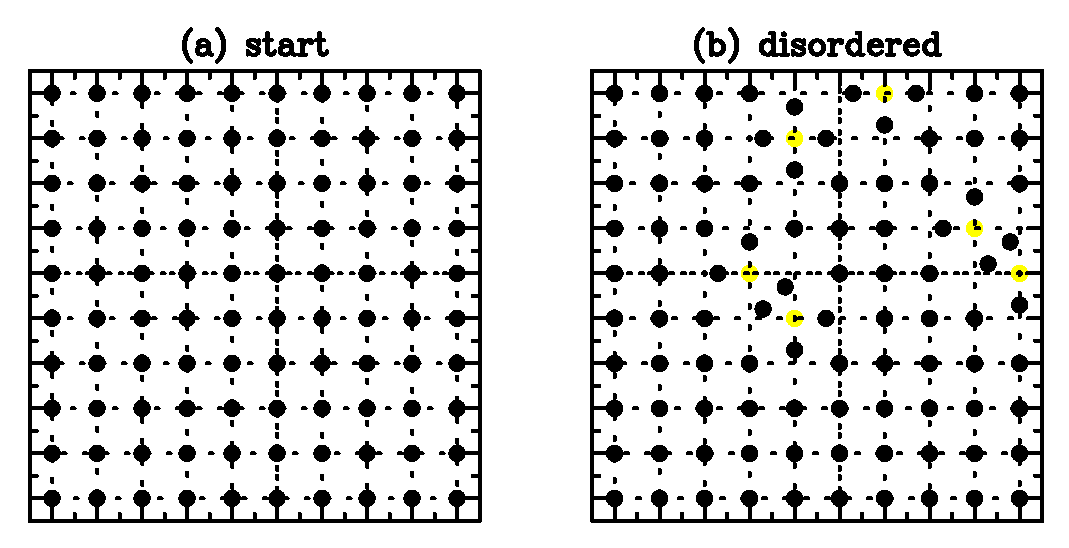
\includegraphics[scale=0.9, angle=0]{mod1.1.eps}
   \caption{Structures created by crystal modification example}
   \label{mod1-fig1}
\end{figure}
%
Here is the macro used to create the described defects.  Again the
line numbers are only shown for convenience and not part of the
macro itself. To achieve a high degree of flexibility values like
crystal size or the number of defects to be created are stored in
variables at the beginning of the macro.  The desired crystal size
is stores in variables i[1], i[2] and i[3] (lines 1-3).  The
variable i[4] (line 5) gives the number of defects to be created
and r[1] (line 6) specifies the relaxation (here 30 \%) of the
surrounding neighbors towards the vacant site.
%
\begin{MacVerbatim}
     1  i[1] = 10
     2  i[2] = 10
     3  i[3] = 1
     4  #
     5  i[4] = 6
     6  r[1] = 0.30
     7  #
\end{MacVerbatim}
%
Next we read the unit cell from file {\it cell.cll} and expand it to
the desired size (lines 8-9).  The macro {\it plot.mac} (line 11)
saves the starting structure suitable for plotting with {\it KUPLOT}
as seen in figure \ref{mod1-fig1}a).
%
\begin{MacVerbatim}
     8  read
     9  cell cell.cll,i[1],i[2],i[3]
    10  #
    11  @plot before.plot
    12  #
\end{MacVerbatim}
%
The next part (lines 13-15) is needed to switch off periodic crystal
boundaries for the command {\tt find} (line 24), otherwise our
simple way of relaxing the neighbors would not work.
%
\begin{MacVerbatim}
    13  chem
    14  set mode,quick,noperiodic
    15  exit
\end{MacVerbatim}
%
Now the creation of the disordered structure starts with a loop over
the number of defects to be created (line 19).  Next a crystal site
is chosen at random (line 20).  Note that the function {\tt ran(0)}
produces a random number between 0 and 1 which is multiplied with
the number of atoms within the crystal (n[3] contains the number of
atoms per unit cell, see table \ref{v1-tab} in section \ref{get}).  
If an occupied site
was picked (line 22) the atom is removed (line 23).  The command
{\tt find} (line 24) returns all atoms of the type Zr around the
position of the selected site within a radius of 5.5\AA.  The atom
indices of these nearest neighbors are stored in the variables {\tt
env[$<$i$>$]} and {\tt env[0]} contains the number of found
neighbors. Finally the positions of all neighboring atoms returned
by {\tt find} are moved towards the vacant site (lines 27-29).
%
\begin{MacVerbatim}
    16  #
    17  # Loop number of wanted defects
    18  #
    19  do i[5]=1,i[4]
    20    i[6]=int(ran(0)*i[1]*i[2]*i[3]*n[3])+1
    21  #
    22    if(m[i[6]].eq.1) then
    23      m[i[6]]=0
    24      find env,zr,x[i[6]],y[i[6]],z[i[6]],5.5
    25  #
    26      do i[7]=1,env[0]
    27        x[env[i[7]]]=x[env[i[7]]]-r[1]*(x[env[i[7]]]-x[i[6]])
    28        y[env[i[7]]]=y[env[i[7]]]-r[1]*(y[env[i[7]]]-y[i[6]])
    29        z[env[i[7]]]=z[env[i[7]]]-r[1]*(z[env[i[7]]]-z[i[6]])
    30      enddo
    31  #
    32    endif
    33  #
    34  enddo
    35  #
    36  @plot after.plot
\end{MacVerbatim}
%
The resulting structure can be seen in figure \ref{mod1-fig1}b.
The introduced vacancies are shown as yellow circles (or light
grey). Since this simple macro does not check whether neighboring
atoms are already displaced, the clustered defects in the upper
right quadrant of figure \ref{mod1-fig1}b have a different local
environment compared to the isolated defects.

%------------------------------------------------------------------------

\section{Build in functions \label{mod-buildin}}

This section will give an overview of those \Discus functions
modifying single atoms or molecules.  Some of these functions can be
realized using variables as well, others cannot like the command
{\tt insert} to insert a new atom in the model crystal.  Table
\ref{mod-tab-1} summarizes the available commands.
%
\begin{table}[!tbh]
\centering
\begin{tabularx}{\textwidth}{|p{30mm}|X|}
  \hline
  {\bf Command} & {\bf Description} \\
  \hline\hline
  append  & Appends an atom at a given position within the crystal if
            no other atoms are present in a given distance.\\
  copy    & Copies an atom to a different position given absolute or
            relative to the other position.\\
  insert  & Inserts a new atom at the given position without condition.\\
  kick    & Inserts a new atom at a given position and removes all
            other atoms within a given distance from the new atom.\\
  remove  & Removes an atom or molecule from the crystal.\\
  switch  & Swaps two given atoms or molecules within the crystal.\\
  purge   & Removes vacancies (VOID) from the crystal ({\bf use with
            care})\\
  replace & Replaces one or more atoms or molecules with the given
            type.\\
  \hline
\end{tabularx}
\caption{\label{mod-tab-1}\Discus commands for single atoms or
         molecules}
\end{table}
%
Basically there are three commands to insert a new atom in the
structure. The command {\tt insert} just creates a new atom at a
specified position without taking notice of its environment. Thus
the new atom might be on top of an existing one. In order to avoid
this problem, \Discus provides two other commands {\tt append}
which will not insert the atom if there are other atoms within a
given distance and {\tt kick} which will remove those atoms close by
before inserting the new one. The command {\tt copy} allows the user
to copy an existing atom to a new position that can be given in
absolute coordinated or relative to the position of the atom to be
copied. Note, that these commands are limited to atoms. New molecule
types can be created and molecules copied using the generalized
symmetry segment of \Discus described in chapter
\ref{cryst-sym}. \par

The commands {\tt remove} and {\tt switch} work for atoms as well as
molecules. Not surprisingly, {\tt remove} removes an atom or
molecule and {\tt switch} swaps two atoms or molecules with respect
to their location within the crystal. \par

The commands mentioned in this section so far operate only on a
single atom or molecule. The command {\tt replace} can replace a
single atom or molecule by a given type or replace more until a
given concentration is reached. Although this can be easily realized
using the FORTRAN interpreter and variables associated with the
crystal, the internal function is much faster, especially for large
crystal sizes. The command {\tt purge} will remove all vacancies
(VOID) within the crystal. Note that if you remove an atom or a
molecule by the {\tt remove} command, \Discus will not actually
remove atoms but rather replace their atom type with VOID. Thus when
saving the structure a large number of VOID's might appear in the
number. The use of {\tt purge} actually removes those VOID atoms.
However, the use of the {\tt purge} command is {\bf not recommended}
since many \Discus function require the crystal to be build in
a given order, i.e. having the same number of atom sites within
every unit cell either occupied by an atom or a VOID.

%------------------------------------------------------------------------

\section{Inserting extended objects \label{mod-insert}}

In order to insert extended objects for small angle scattering or
domains \ref{mod-domain} \Discus offers an insert menu. In contrast
to the insert command for individual atoms, the menu is evoked by
the {\tt insert} command followed by the keyword {\tt domain} or
{\tt object}. A corresponding version for molecules is under
construction. 

\subsection{Inserting domains \label{mod-insdom}}

Within the \Discus formalism, a domain (see section 
\ref{mod-domain} for a full explanation ) is 
essentially a molecule which will be interpreted differently. 
The domain allows you to place an extended defect into a host 
structure. The {\tt insert domain} menu allows you to specify
the character and location of the domain to be inserted.
%------------------------------------------------------------------------
